\documentclass[12pt, a4paper, lithuanian]{article}
\usepackage[utf8x]{inputenc}
\def\LTfontencoding{L7x}
\PrerenderUnicode{ąčęėįšųūž}
\usepackage[\LTfontencoding]{fontenc}
\usepackage[lithuanian]{babel}
\usepackage{VUMIFPSkursinis}
\usepackage{cite}
\usepackage{amsmath}
\usepackage{bm}
\usepackage{amsfonts}
\usepackage{float}
\usepackage{graphicx}
\usepackage{color}
\usepackage{listings}
\usepackage{wrapfig}
\usepackage{algpseudocode}
\usepackage{algorithm}
\usepackage{algorithmicx}
\usepackage{caption}
\usepackage{subfig}


% Titulinio aprašas
\vumifdept{Programų sistemų katedra}
\vumifpaper{Kursinis darbas}
\title{Biojutiklio su selektyvia membrana kompiuterinis modeliavimas}
% \title{Esama situacija su dviem sluoksniais}
% \title{Ištirti selektyvios membranos įtaką amperometrinio bijojutiklio jautriui}
\def\titleineng{*angl. pav.}
\def\statusas{% Kai kurioms katedroms reikia nurodyti  
    4 kurso 1 grupės studentas \\
}
\author{
   Kęstutis Gimbutas
}

\supervisor{prof. habil. dr. Romas Baronas}
\date{Vilnius – \the\year}

\begin{document}
\sloppy
\maketitle

\tableofcontents

\sectionnonum{Įvadas}
\textit{<Tektas>} \textbf{*}.

\section{Biojutiklio su selektyvia membrana modelis}
Sudarant modelius bei lygtis buvo pasinaudota šaltiniais:
\cite{baronas2009mathematical}, \cite{baronas2006computational},
\cite{baronas2003influence}.

\subsection{Matematinis modelis}
Remiantis supaprastinta schema koncentratas (S) prisijungia prie fermento (E)
ir yra
paverčiamas į produktą (P),
\begin{equation}\label{eq:basic} 
    S \overset{E}{\rightarrow} P
\end{equation}

Biojutiklio veikimo sistemos lygiai: koncentratas, fermento sluoksnis($\Omega_2$),
selektyvios
membranos sluoksnis($\Omega_1$), elektrodas.
\begin{equation}
    \frac{\delta P_1}{\delta t} = D_{1P} \frac{\delta^2 P_1}{\delta x^2}, \;
    kai\; x \in \Omega_1,\;\; t > 0.
\end{equation}

\begin{equation}
\begin{aligned} 
    &\frac{\delta S}{\delta t} = D_S \frac{\delta^2 S}{\delta x^2} -
    \frac{V_{max} S}{K_M + S}, \; kai\; x \in \Omega_2,\;\; t > 0.  \\ 
    &\frac{\delta P_2}{\delta t} = D_{2P} \frac{\delta^2 P_2}{\delta x^2} +
    \frac{V_{max} S}{K_M + S}, \; kai\; x \in \Omega_2 ,\;\; t > 0.
\end{aligned}
\end{equation}


\subsection{Pradinės ir kraštinės sąlygos}
\begin{equation}
\begin{aligned}
    &S(x, 0) = 0,\; x \in \Omega_2,\\
    &S(d, 0) = S_0,
\end{aligned}
\end{equation}

\begin{equation}
\begin{aligned}
    &P_1(x, 0) = 0,\; x \in \Omega_1,\\
\end{aligned}
\end{equation}

\begin{equation}
\begin{aligned}
    &P_2(x, 0) = 0,\; x \in \Omega_2,\\
    &P_2(d, 0) = P_0,
\end{aligned}
\end{equation}

\begin{equation} 
    P_1(0;t)=0, \; t>0.
\end{equation}

\begin{equation} 
    \left. D_S \frac{\delta S}{\delta x} \right|_{x=0} = 0, t>0.
\end{equation}

\begin{equation} 
    S(d, t) = S_0,\; t>0,
\end{equation}

\begin{equation} 
    P_2(d, t) = 0,\; t>0.
\end{equation}

\subsection{Biosensoriaus atsako charakteristikos}
\subsubsection{Atsako laikas}
\begin{equation} 
\begin{aligned}
    T = \underset{i(t)>0}{min}\left\{t:\frac{t}{i(t)} \left| \frac{d_i(t)}{dt}
    \right| < \epsilon \right\}
\end{aligned}
\end{equation}

\subsection{Skaitinis lygčių aproksimavimas}
\subsubsection{Neišreikštinė schema}

\begin{equation}
\begin{aligned} 
    &\frac{S_i^{j+1} - S_i^j}{\tau} = D\frac{S_{i+1}^{j+1} -
    2S_i^{j+1} + S_{i-1}^{j+1}}{h^2} -
    \frac{V_{max} S_i^j}{K_M + S_i^j},\\ 
    &\frac{P_i^{j+1} - P_i^j}{\tau} = D\frac{P_{i+1}^{j+1} -
    2P_i^{j+1} + P_{i-1}^{j+1}}{h^2} +
    \frac{V_{max} S_i^j}{K_M + S_i^j},\\ 
    &i = 1,\;...,\; N-1,\; j=0,\;...,\;M-1.
\end{aligned}
\end{equation}

\subsubsection{Pradinės ir kraštinės modelio sąlygos}
\begin{equation}
\begin{aligned}
    &S_i^0 = 0, i = 0,\;...,\;N-1,\\
    &S_N^0 = S_0,
\end{aligned}
\end{equation}

\begin{equation}
\begin{aligned}
    &P_i^0 = 0, i = 0.\;...,\;N-1,\\
    &P_N^0 = P_0
\end{aligned}
\end{equation}

\begin{equation} 
    S_0^j = S_1^j, S_N^j = S_0, j=1,\; ...,\;M, 
\end{equation}

\begin{equation} 
    P_0^j = 0, P_N^j = P_0, j=1,\; ...,\;M, 
\end{equation}

\subsubsection{Skaičiavimo procedūra}

\begin{equation} 
    i(t_j) \approx t_j = n_eFD_pP_i^j/h,\; j=1,\;...,\;M. 
\end{equation}

\subsection{Skaitinio sprendimo tikrinimas}
\subsubsection{Pradinės skaičiavimų sąlygos}

\begin{equation}
\begin{aligned}
    &S_0 = 1 \mathrm{\mu M},\; P_0 = 0 \mathrm{\mu M},\\
    &D_s = 300 \mathrm{\mu m^2/s},\; D_p = 300 \mathrm{\mu m^s/s},\\
    &T = 50\mathrm{s},\;\; d_1 = 10 \mathrm{\mu m},\; d_2 = 15\mathrm{\mu m},\; d_3 = 100\mathrm{\mu m}; d_4 =
    150\mathrm{\mu m},\\
    &\tau = 0.1\mathrm{s},\; h=0.1 \mathrm{\mu m},\\
    &V_{max} = 100\mathrm{\mu M /s},\; \epsilon = 0.05,\\
    &F=961485,\; K_M= 100\mathrm{\mu M},\; n_e = 2.
\end{aligned}
\end{equation}

\subsubsection{Gautos matricos iš neišreikštinės schemos}
\textit{Lygčių sistemos gautos naudojant baigtinių skirtumų medodą ir neišreikštines schemas. Lygtys išsprėstos taikant triįstrižainių matricų algoritmą.}
\begin{equation}
\left\{
\begin{aligned}
    &S_{i+1}^{j+1}-S_i^{j+1}\left(1+\frac{h^2}{D\tau}\right)
= \frac{h^2}{D\tau} \left(\frac{V_{max}S_i^j\tau}{K_M+S_i^j}-S_i^j\right),\; kai \; i = 1,\\
    &\dots\;,\\
    &S_{i-1}^{j+1}-S_i^{j+1}\left(2+\frac{h^2}{D\tau}\right)+S_{i+1}^{j+1}
        = \frac{h^2}{D\tau}
        \left(\frac{V_{max}S_i^j\tau}{K_M+S_i^j}-S_i^j\right),\; kai\; i =
        2,\;...,\;N-1,\\
    &\dots\;,\\
    &S_0 + S_{i-1}^{j+1} - S_i^{j+1}\left(2+\frac{h^2}{D\tau}\right)
        =  \frac{h^2}{D\tau}
    \left(\frac{V_{max}S_i^j\tau}{K_M+S_i^j}-S_i^j\right),\; kai \; i = N.
\end{aligned}
\right.
\end{equation}

\begin{equation}
\left\{
\begin{aligned}
    &P_{i+1}^{j+1}-P_i^{j+1}\left(2+\frac{h^2}{D\tau}\right)
    = \frac{h^2}{D\tau} \left(-P_i^j -\frac{V_{max}S_i^j\tau}{K_M+S_i^j}\right),\; kai \; i = 1,\\
    &\dots\;,\\
    &P_{i-1}^{j+1}-P_i^{j+1}\left(2+\frac{h^2}{D\tau}\right)+P_{i+1}^{j+1}
        = \frac{h^2}{D\tau}
    \left(\frac{V_{max}S_i^j\tau}{K_M+S_i^j}-S_i^j\right),\; kai\; i =
        2,\;...,\;N-1,\\
    &\dots\;,\\
    &P_0 + P_{i-1}^{j+1} - P_i^{j+1}\left(2+\frac{h^2}{D\tau}\right)
        =  \frac{h^2}{D\tau}
        \left(\frac{V_{max}S_i^j\tau}{K_M+S_i^j}-S_i^j\right),\; kai\; i = N.
\end{aligned}
\right.
\end{equation}

\subsubsection{Rezultatai}

\begin{figure}[H]
    \centering
    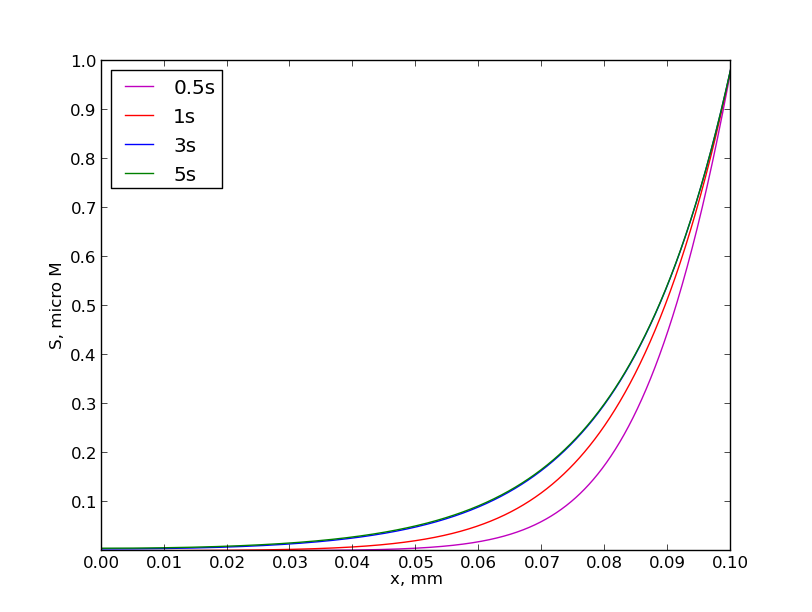
\includegraphics[scale=0.5]{img/S}
    \caption{Substrate}
    \label{img:mlp}
\end{figure}

\begin{figure}[H]
    \centering
    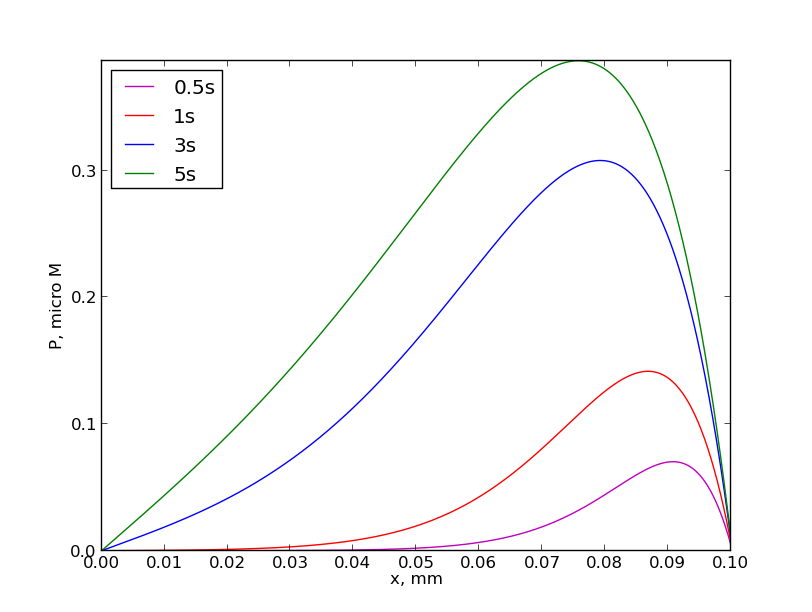
\includegraphics[scale=0.5]{img/P}
    \caption{Product}
    \label{img:mlp}
\end{figure}

\begin{figure}[H]
    \centering
    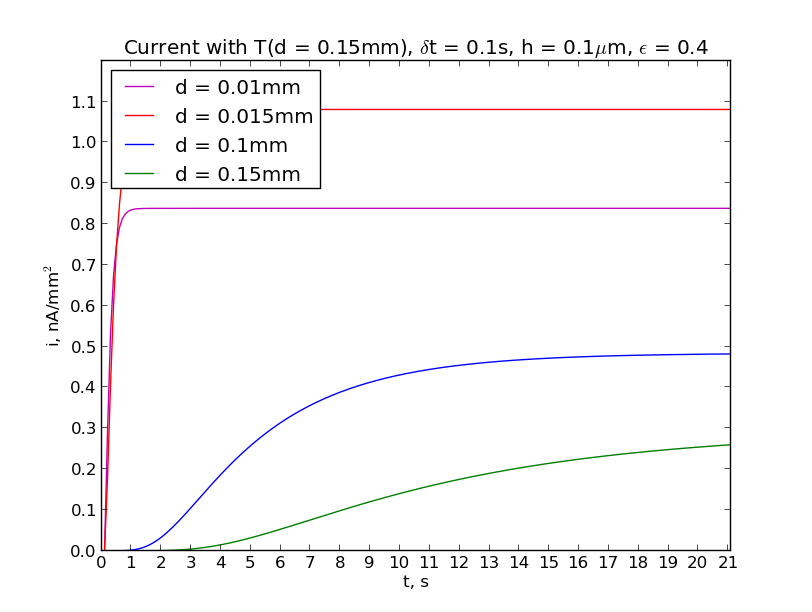
\includegraphics[scale=0.5]{img/i}
    \caption{Current}
    \label{img:mlp}
\end{figure}

%\appendix
%----------------------------------------------------

\bibliography{bibliografija}


%\appendix
%\section{Papildomų eksperimentų rezultatų lentelės}
%\begin{figure}[H]
%    \centering
%    \includegraphics[scale=0.5]{img/MLP}
%    \caption{Paveikslėlio pavyzdys}
%    \label{img:mlp}
%\end{figure}
%
\end{document}
